\chapter{Results}\label{chap:res}

In this section I present the main results from the analysis. The effects of the relevant experimental variables are evaluated with a logistic regression, and the adjusted $\lambda$ is discussed at different levels of aggregation.

\section{Descriptive Statistics}

% report raw descriptive statistices of payoffs and entrnce, as is costum in regression analysis (use stargazer)

There are at most two possible equilibria in pure strategies in each game. However, many other profiles occurred. 
Table \ref{playedStrategies} shows the proportion each configuration was played by game.
First columns display the eight possible profiles. For example, profile 3 ($[0, 1, 0]$) means that only citizen $q_{30}$ enter the competition. 
This profile is a SNE in all games, and is the most frequent in RO games.
Notice that the more frequent profiles are 3 and 4 in $PR\_HC$ game and, 4 and 8 in the $PR\_LC$.
This phenomena can be explained first because citizen $q_{80}$ wins in most scenarios where others deviate from equilibrium; and second because, with low costs, citizen $q_{20}$ face the same logic and then profile 8 (every citizen campaign) increases its probability. % relate with Harsanyi's equilibrium selection
This kind of considerations are captured by the QRE theory. 

% Table created by stargazer v.5.2 by Marek Hlavac, Harvard University. E-mail: hlavac at fas.harvard.edu
% Date and time: jue., abr. 27, 2017 - 09:48:31 p. m.
\begin{table}[!htbp] \centering  
	\begin{tabular}{@{\extracolsep{5pt}} cccccccc} 
		\\[-1.8ex]\hline 
		\hline \\[-1.8ex]
		& \multicolumn{3}{c}{Profiles} & \multicolumn{4}{c}{Games} \\
		\hline \\[-1.8ex]
		& 20 & 30 & 80 & PR\_LC & PR\_HC & RO\_LC & RO\_HC \\ 
		\hline \\[-1.8ex] 
		1 & $0$ & $0$ & $0$ & $0.013$ & $0.029$ & $0.006$ & $0.020$ \\ 
		2 & $0$ & $0$ & $1$ & $0.048$ & $0.066$ & $0.003$ & $0.006$ \\ 
		3 & $0$ & $1$ & $0$ & $0.067$ & \textbf{0.305} & \textbf{0.347} & \textbf{0.589} \\ 
		4 & $0$ & $1$ & $1$ & \textbf{0.402} & \textbf{0.366} & \textbf{0.252} & \textbf{0.151} \\
		5 & $1$ & $0$ & $0$ & $0.009$ & $0.013$ & $0.008$ & $0.011$ \\ 
		6 & $1$ & $0$ & $1$ & $0.063$ & $0.018$ & $0.011$ & $0.000$ \\ 
		7 & $1$ & $1$ & $0$ & $0.044$ & $0.079$ & $0.210$ & $0.146$ \\ 
		8 & $1$ & $1$ & $1$ & \textbf{0.354} & $0.124$ & $0.164$ & $0.077$ \\ 
		\hline \\[-1.8ex] 
		\multicolumn{4}{r}{Total trials:} & $540$ & $380$ & $648$ & $350$ \\ 
		\hline \\[-1.8ex] 
	\end{tabular} 
	\caption[Proportion of played strategies]{For each game, the proportions of the eight possible combinations of strategies played are shown ($1:entry$, $0:abstain$). The total number of actual trials are set at the bottom.}
	\label{playedStrategies}
\end{table} 

It is important to review the aggregated proportion of entrance by ideal point precisely because these proportions are the direct prediction of QRE theory. Table \ref{propEntrance} displays these proportions by game. This table makes clear that once a participant was assigned the ideal point 30, it is quite probable for her to enter. The probability of enter being 80 increases until reach 30's in the $PR\_LC$ condition precisely for de reason explained above. 

% Table created by stargazer v.5.2 by Marek Hlavac, Harvard University. E-mail: hlavac at fas.harvard.edu
% Date and time: vie., abr. 28, 2017 - 12:04:23 a. m.
\begin{table}[!htbp] \centering 
	\begin{tabular}{@{\extracolsep{5pt}} ccccc} 
		\\[-1.8ex]\hline 
		\hline \\[-1.8ex] 
		& PR\_LC & PR\_HC & RO\_LC & RO\_HC \\ 
		\hline \\[-1.8ex] 
		20 & $0.470$ & $0.234$ & $0.392$ & $0.234$ \\ 
		30 & $0.867$ & $0.874$ & $0.972$ & $0.963$ \\ 
		80 & $0.867$ & $0.574$ & $0.429$ & $0.234$ \\ 
		\hline \\[-1.8ex] 
	\end{tabular} 
	\caption[Entry proportion by player]{Proportion of entry by type of player.}
	\label{propEntrance}
\end{table} 

Figure \ref{fig:boxplots} displays the boxplots of the entrance proportion. It can be seen a clear tendency to enter when participants were chosen to be $q_{30}$. The entrance is less for any other ideal point and, in general, with less variability. The most interesting observation is in condition $PR\_LC$ where entrance is equal between $q_{30}$ and $q_{80}$, as shown in table \ref{propEntrance}, and the median is even higher for $q_{80}$.

\begin{figure}
	\centering
	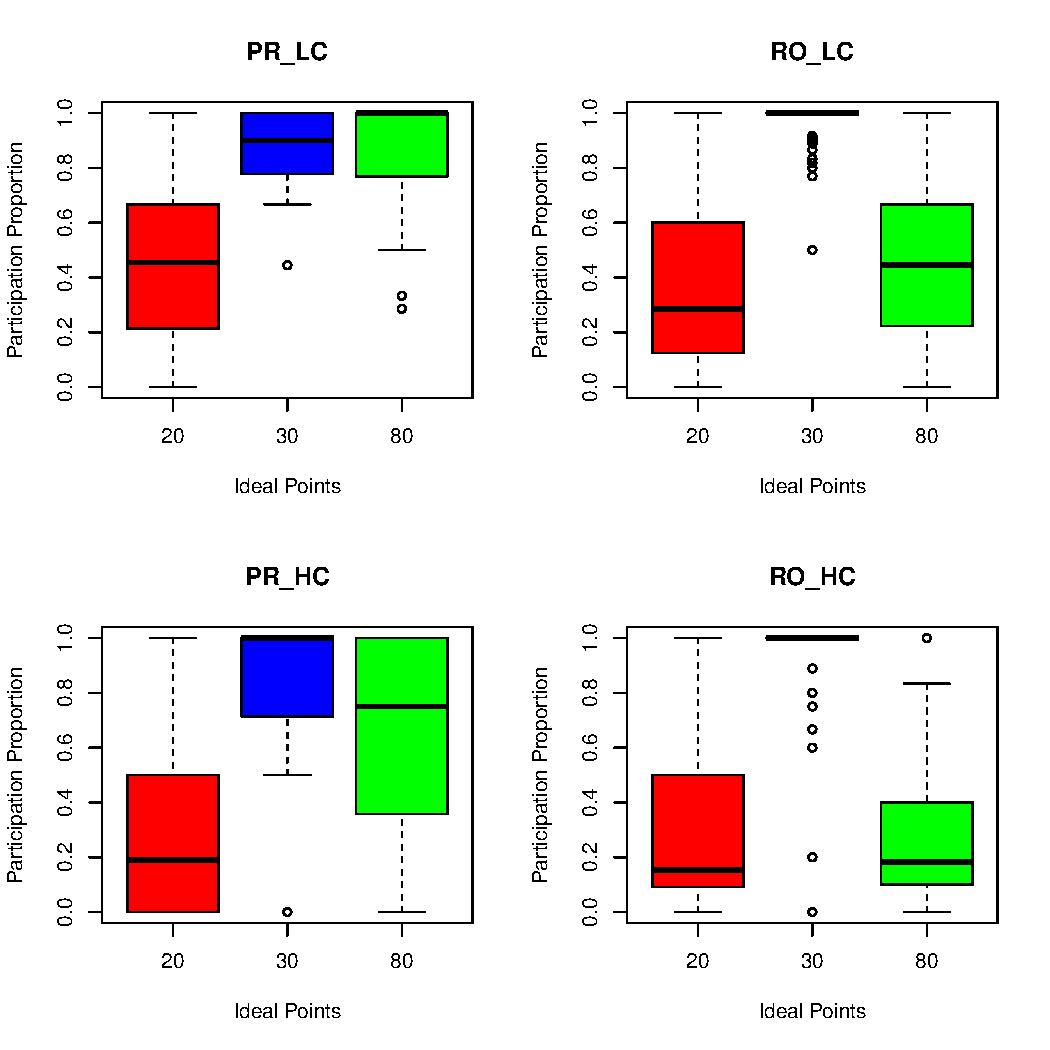
\includegraphics[width=1\linewidth]{../../data/IndividualProportionByGame_boxplot}
	\caption[Boxplots Proportions]{Proportion of entrance by game and by ideal points.}
	\label{fig:boxplots}
\end{figure}

\subsection{Logistic Regression}

In order to evaluate the effect of costs, voting rule, and if there are some difference in proportions through time, I run a logistic regression with random effects using the \emph{lme4} package \cite{Bates2014}. Table \ref{tab:logit_reg} shows\footnote{This table was made with the help of \emph{stargazer} package \cite{Hlavac2015}.} the results from three regressions for each ideal point.

\textit{Period} is a dummy variable -as the other ones- constructed from trials, it split them in two: first 14 trials and the rest. Final number of trials was different for each participant because it depends on the random matchings and bankruptcy, the more equitable distribution is reached with 14 trials for period zero. The effect of this variable is robust across ideal points, which shows that, through time, players tend towards NE: $q_{30}$ campaigning alone. 
%For the rest variables, the same effect's direction is observed

The results confirm statistically the visual analysis made with figure \ref{fig:boxplots}: there is an effect of high cost and RO system towards NE. Additionally, there is no effect of costs over $q_{30}$ possibly due to a ceiling effect -they almost always participate-, for $q_{20}$ there is not effect by election system. Finally, it is worth noting that $q_{80}$'s entrance rate is very sensible to the relevant variables.

% Table created by stargazer v.5.2 by Marek Hlavac, Harvard University. E-mail: hlavac at fas.harvard.edu
% Date and time: vie., abr. 28, 2017 - 12:07:08 a. m.
\begin{table}[!htbp] \centering 
	\begin{tabular}{@{\extracolsep{5pt}}lccc} 
		\\[-1.8ex]\hline 
		\hline \\[-1.8ex] 
		& \multicolumn{3}{c}{\textit{Dependent variable:}} \\ 
		\cline{2-4} 
		\\[-1.8ex] & \multicolumn{3}{c}{Entry} \\ 
		& 20 & 30 & 80 \\ 
		\\[-1.8ex] & (1) & (2) & (3)\\ 
		\hline \\[-1.8ex] 
		HighCost & $-$1.221$^{***}$ & 0.072 & $-$1.875$^{***}$ \\ 
		& (0.277) & (0.321) & (0.284) \\ 
		RunOff & $-$0.199 & 1.896$^{***}$ & $-$2.862$^{***}$ \\ 
		& (0.269) & (0.348) & (0.293) \\ 
		Period & $-$0.984$^{***}$ & 1.118$^{***}$ & $-$1.922$^{***}$ \\ 
		& (0.133) & (0.221) & (0.154) \\ 
		Constant & 0.237 & 2.043$^{***}$ & 3.695$^{***}$ \\ 
		& (0.236) & (0.277) & (0.294) \\ 
		\hline \\[-1.8ex] 
		Observations & 1,918 & 1,918 & 1,918 \\ 
		Akaike Inf. Crit. & 2,028.730 & 908.160 & 1,795.807 \\ 
		Bayesian Inf. Crit. & 2,056.525 & 935.955 & 1,823.602 \\ 
		\hline 
		\hline \\[-1.8ex] 
		\textit{Note:}  & \multicolumn{3}{r}{$^{*}$p$<$0.1; $^{**}$p$<$0.05; $^{***}$p$<$0.01} \\ 
	\end{tabular} 
	\caption{Logistic Regression with Random Effects}
	\label{tab:logit_reg} 
\end{table} 

\section{Maximum Likelihood Estimation}

Data analysis at different levels was calculated by maximum likelihood, following directions from \citeA{Goeree2016}. 
The equilibrium correspondence approach was used: the QRE is calculated for a given $\lambda$ and other parameters ($\beta$): $\sigma*_{ij}(\lambda, \beta)$. In order to find this function, a non linear equations system with no analytical solution has to be solved. 
This was done using the R package \emph{nleqslv} \cite{Hasselman2011}.

Once this function is constructed, it is possible to find the general logLikelihood objective function, and the then optimize it.

\begin{equation}
	logL(\lambda) = 
	\Sigma^n_{i=1} \Sigma^{J_i}_{j=1} f_{i,j} log(\sigma^*_{ij}(\lambda, \beta))
\end{equation}\label{fn:MLE}

In the objective function \ref{fn:MLE}: $n=3$, $J_i = 2$ and $f_{i,j}$ are the times each i-th citizen choose their j-th option.

\subsection{Global Analysis}
In this level, it is considered that every player has the same $\lambda$. Then, the resulting objective function considers the likelihood in each game according with equation \ref{eq:MLE}.

\begin{equation} \label{eq:MLE}
	logL(\lambda) = 
	\Sigma^4_{g=1} \Sigma^n_{i=1} \Sigma^{J_i}_{j=1} f_{g,i,j} log(\sigma^*_{ij}(\lambda, \beta_g))
\end{equation}

Parameter $\beta_g$ refers to the payoffs in the g-th game, and it is clear that the estimated equilibrium depends on the payoffs. The $\lambda$ estimated this way is $ 0.0782$. This result and those for the analysis by game are shown in the table \ref{mle_lambda}.

% latex table generated in R 3.3.3 by xtable 1.8-2 package
% Thu Apr 06 10:47:12 2017
\begin{table}[ht]
	\centering
	\begin{tabular}{rrrrrr}
		\hline
		& Global & PR\_LC & PR\_HC & RO\_LC & RO\_HC \\ 
		\hline
		$\lambda$ & 0.0782 & 0.0836 & 0.0723 & 0.0984 & 0.0832 \\ 
		\hline
	\end{tabular}\caption[MLE: global and by game]{MLE of $\lambda$ for the global analysis and for each game.}\label{mle_lambda}
\end{table}

\subsection{Game Analysis}

It could be possible to observe an effect by game over $\lambda$ which would imply that it is a function of payoffs. For this reason rationality parameter is calculated by game and compared with global result.

In the figure \ref{fig:qrelambdamle}, it is possible to compare the aggregated adjustment in each game. This graph shows soft lines which state the predicted rate of entrance for each citizen type as a function of $\lambda$. The vertical lines are located at the adjusted $\lambda$; solid and dashed lines are in global and by game calculation respectively. Horizontal lines are located at the proportions observed in data, they used the same color pattern for each ideal point than in soft lines. 

\begin{figure}
	\centering
	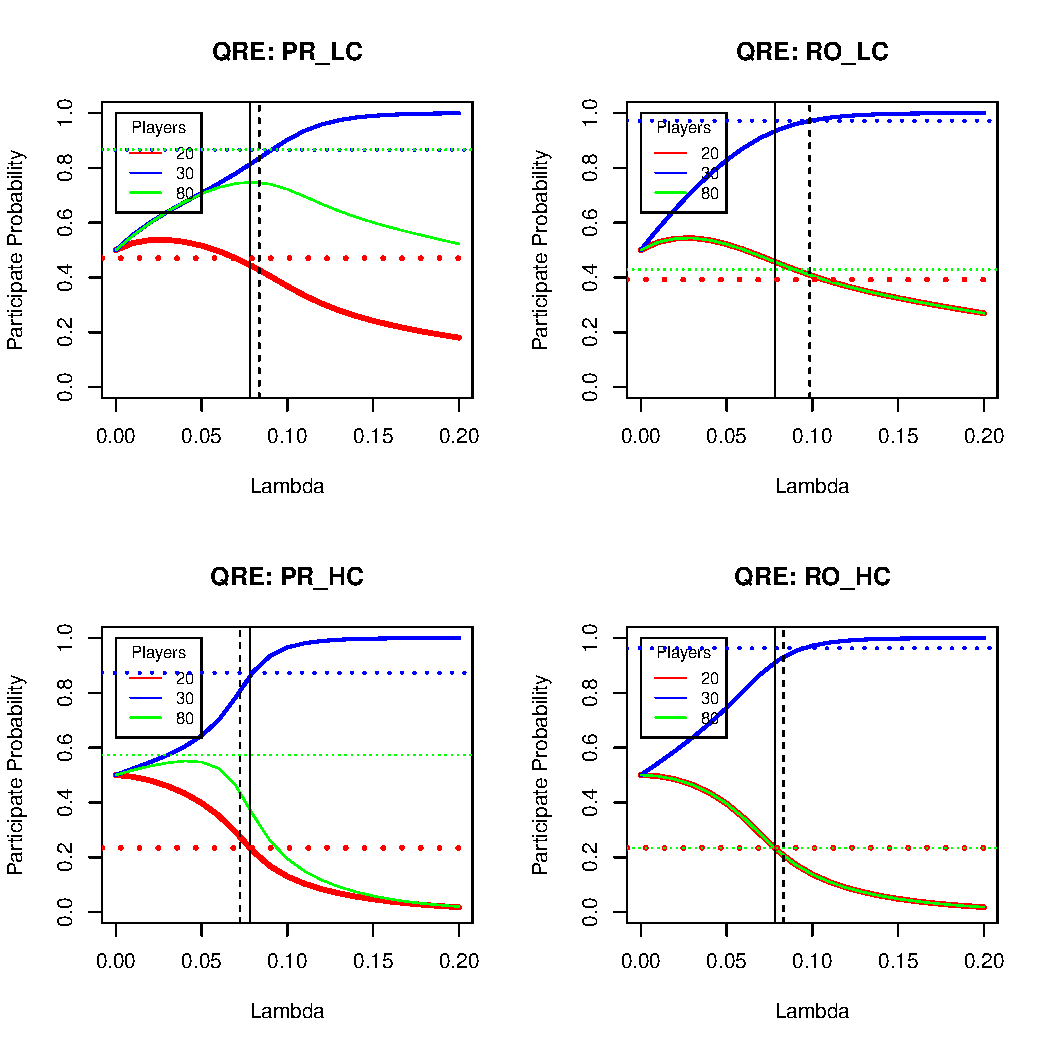
\includegraphics[width=1\linewidth]{../../data/QRE_lambda_MLE}
	\caption[QRE]{Equilibria for different Lambda}
	\label{fig:qrelambdamle}
\end{figure}

It is clear from figure \ref{fig:qrelambdamle} that there are no large differences between the global and by game estimates and that predictions from both (vertical and smooth lines intersections) are close to the observed proportions.

There is always heterogeneity in the participants that can be interesting to observe and measure. For this reason the analysis by individual is included.

\subsection{Individual Analysis}

In figure \ref{fig:individualproportionbygame} it is possible to observe the heterogeneity across and inside the games. 
Red lines represent entrance rates of those participants who end in bankruptcy before the programed trials ended. First, it is clear that the logit equilibrium is the more frequent strategy played across participants.
Also, there is observed heterogeneity across games in this respect that could be explained by the payoffs, because a mistake in high cost games is more important. 
This heterogeneity cannot be explained by a more random behavior in high cost games considering that $\lambda$ estimations are not too much different across games -as can be seen in figure \ref{fig:qrelambdamle}. There is the possibility of a biased measure of the strategies played in this games due to the fact that more  random participants, who are more prone to bankruptcy, played less trials than more rational participants. For this reason it is important to analyze individuals in a more detailed way. 

\begin{figure}
	\centering
	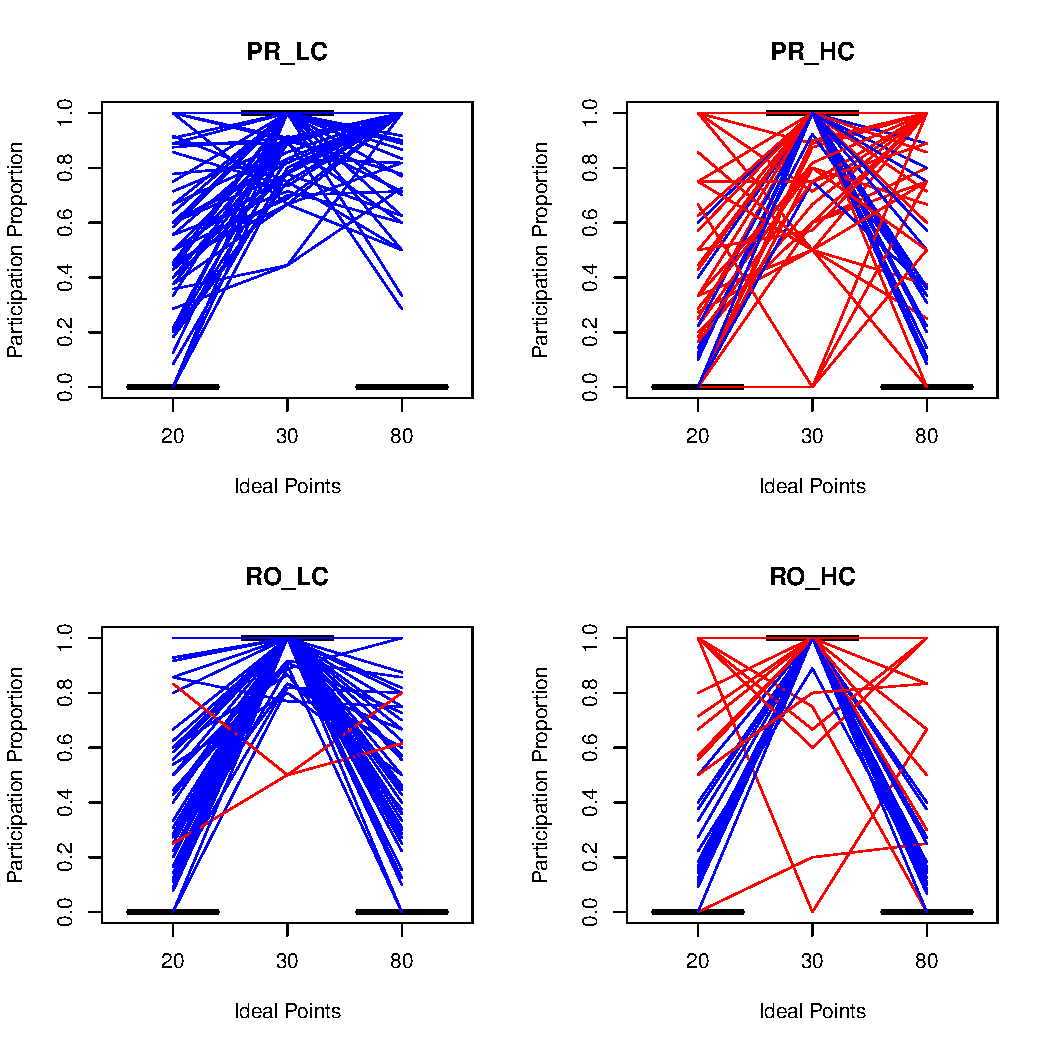
\includegraphics[width=0.7\linewidth]{../../data/IndividualProportionByGame}
	\caption[Individual Proportions]{Each line connects the proportion of entry when a participant played for different ideal points.}
	\label{fig:individualproportionbygame}
\end{figure}

Figure \ref{fig:lambdadistributionbygame} shows the histograms for MLE estimators in each game. They were calculated in a slight different way than \citeA{Goeree2016} . In this case, for each player the proportions of their own elections in different ideal points were used to calculate $\lambda$, it is like consider that each participant play against herself.

\begin{figure}
	\centering
	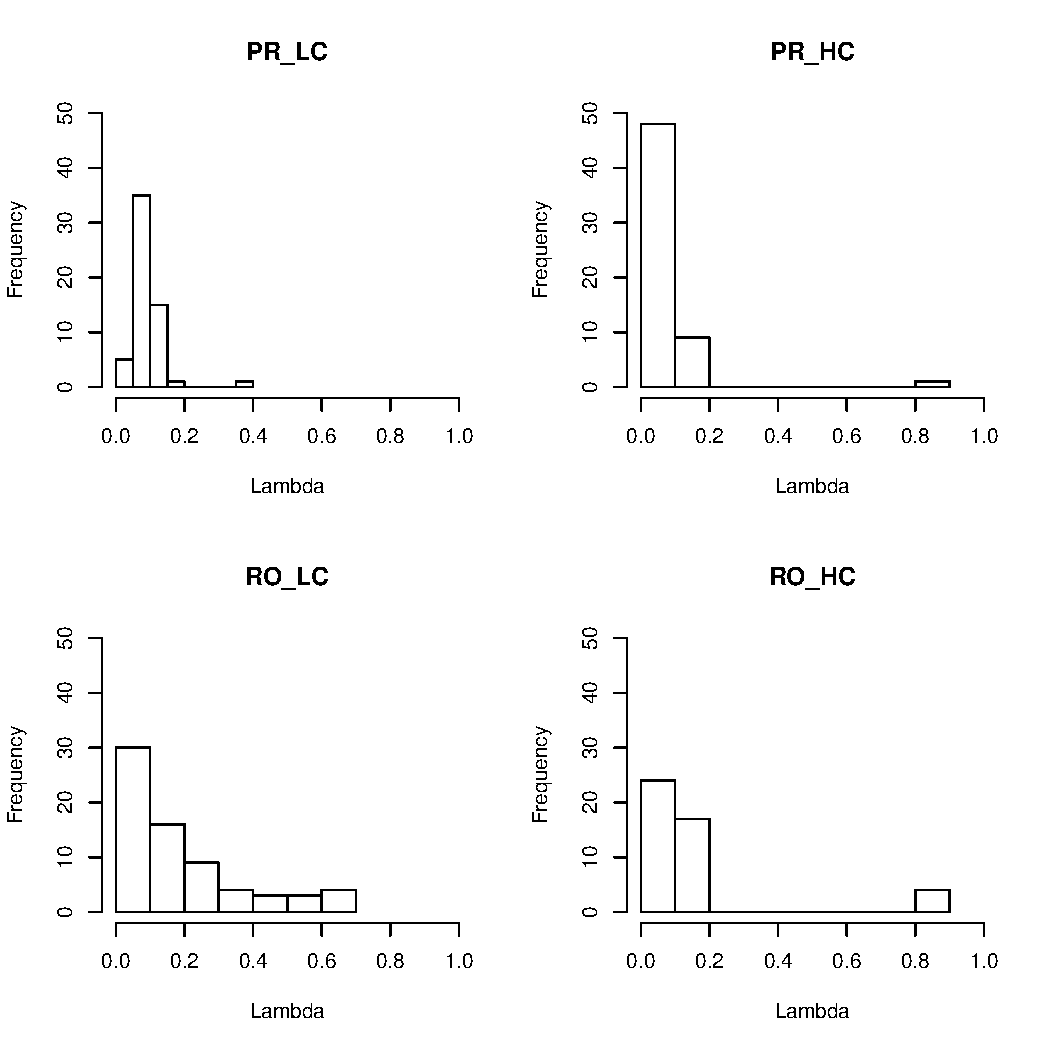
\includegraphics[width=1\linewidth]{../../data/LambdadistributionByGame}
	\caption[Individual Proportions]{Each line connects the proportion of entry when a participant played for different ideal points.}
	\label{fig:lambdadistributionbygame}
\end{figure}


It can be noticed that the distributions are not very different, and could be described by an exponential distribution. For high cost games it is clear that there are a few players that are apart from the main population to the right: maybe those who played the logit equilibrium almost perfectly.

% check for particular prediction at the indovidual level and plot histograms comparing this distribution with observed

